\documentclass[conference]{IEEEtran}

\usepackage[T1]{fontenc}
\usepackage[utf8]{inputenc}
\usepackage{lmodern}
\usepackage{microtype}
\usepackage{amsmath,amssymb,bm}
\usepackage{booktabs,tabularx,array,multirow}
\usepackage{graphicx}
\usepackage{xcolor}
\usepackage{enumitem}
\usepackage{algorithm}
\usepackage{algpseudocode}
\usepackage{tikz}
\usetikzlibrary{arrows.meta,positioning,shapes.geometric,fit}
\usepackage{siunitx}
\usepackage{csquotes}
\usepackage[hidelinks]{hyperref}
\makeatletter
\renewcommand*{\theHALG@line}{\thealgorithm.\arabic{ALG@line}}
\makeatother
\usepackage[nameinlink,noabbrev]{cleveref}
\usepackage[
  backend=biber,
  style=ieee,
  sorting=none,
  giveninits=true,
  doi=true,
  url=true,
  isbn=false,
  maxnames=8,
  minnames=3
]{biblatex}
\addbibresource{references.bib}

\newcommand{\system}{NZ-Edge}
\newcommand{\COtwo}{CO\textsubscript{2}}
\newcommand{\COtwoe}{CO\textsubscript{2}e}
\newcommand{\RQ}[1]{\textbf{RQ#1}}
\newcommand{\HYP}[1]{\textbf{H#1}}
\newcommand{\code}[1]{\texttt{#1}}
\DeclareSIUnit\coTwoEquivalent{kg\,CO_2e}

\title{Edge AI-Enabled Net Zero Management for Campus Buildings Using Qualcomm QIDK: A Research and Implementation Proposal}

\author{\IEEEauthorblockN{Team: esworkingshoppers}
\IEEEauthorblockA{Embedded Systems Workshop\\
Nitya Joshi: 2025111023\\
Teja Pudi: 2025111021\\}}

\begin{document}
\maketitle

\begin{abstract}
	Campus sustainability platforms usually centralize telemetry and display historical energy, water, waste, and environmental indicators. They provide visibility but rarely combine local multimodal inference, uncertainty-aware prediction, verified carbon accounting, and safe real-time control. Their cloud dependence also creates latency, connectivity, bandwidth, privacy, and operational-resilience limitations. This proposal specifies \system{}, an edge-AI platform that executes building forecasting, fault detection, and carbon-aware supervisory optimization on a Qualcomm Innovators Development Kit (QIDK) Android device. The device consumes electricity, photovoltaic, HVAC, indoor-air-quality, occupancy, water, waste, weather, tariff, and grid-carbon data through a segmented protocol gateway. It cannot replace certified building controllers or life-safety systems. The principal control method is constrained model predictive control (MPC), with deterministic limits and fallback sequences independent of learned models. Recent time-series foundation models and graph models are evaluated as challengers, not presumed superior to seasonal and gradient-boosted baselines. Models are quantized and compiled with Qualcomm AI Runtime and QNN for CPU, GPU, and Hexagon NPU comparison. A staged replay, digital-twin, hardware-in-the-loop, shadow, advisory, and randomized field evaluation measures adjusted energy, operational carbon, peak demand, comfort, indoor air quality, availability, privacy, inference latency, and edge-compute energy. Savings follow an IPMVP-style counterfactual and report location- and market-based emissions separately. The central hypothesis is that local, uncertainty-gated supervisory intelligence can reduce operational energy and emissions while preserving occupant service, auditability, privacy, and safe building operation.

\end{abstract}

\begin{IEEEkeywords}
	edge AI, net zero, building energy management, model predictive control, Qualcomm QIDK, carbon-aware computing, fault detection, measurement and verification
\end{IEEEkeywords}

\section{Introduction}

Buildings account for material direct and indirect energy use, greenhouse-gas (GHG) emissions, water withdrawals, and waste generation. A campus compounds the problem: buildings differ in construction, occupancy, schedules, plant topology, metering, and control maturity, while sharing utility connections, central plants, renewable generation, storage, and operational staff. Net-zero management is therefore a cyber-physical problem rather than a dashboard problem. It requires trustworthy measurements, an explicit accounting boundary, forecasts of future demand and conditions, safe decisions under uncertainty, and evidence that an intervention changed physical outcomes relative to what would otherwise have happened.

Most sustainability management products collect data in a central or cloud platform. This is useful for portfolio reporting, but it creates four limitations. First, network delay and service interruption can prevent timely decisions. Second, continuously transmitting fine-grained occupancy or equipment data increases privacy and cybersecurity exposure. Third, centralized processing creates bandwidth and cloud-compute overhead. Fourth, a dashboard that reports consumption does not itself optimize a building or establish that reported savings are causal. Edge computing can address the first three limitations, but it addresses the fourth only when combined with sound control, measurement and verification (M\&V), and governance.

This proposal introduces \system{}, a campus-building platform centered on a Qualcomm QIDK Android device. QIDK denotes the \emph{Qualcomm Innovators Development Kit}, not the QCS6490/RB3 or QRB5165/RB5 embedded platforms. The actual QIDK system-on-chip (SoC), Android build, accelerator generations, and runtime versions will be qualified and recorded before model selection. The design uses Qualcomm AI Runtime (QAIRT), including QNN/Qualcomm AI Engine Direct, to execute compatible quantized models on the available Hexagon neural-processing hardware. Official Qualcomm documentation, rather than nominal tera-operations-per-second figures, will determine supported operations and deployment formats~\cite{qualcomm_qidk,qualcomm_qairect,qualcomm_aihub_compile}.

The research is deliberately energy-led. Electricity, HVAC, on-site photovoltaics (PV), and storage are candidates for guarded supervisory optimization. Water, waste, indoor air quality (IAQ), and occupancy are integrated as multimodal monitoring, prediction, constraint, and anomaly-detection domains. No learned model receives unrestricted building-management-system (BMS) write access. Existing local controllers retain regulation, equipment protection, and life-safety authority.

The proposed contributions are:
\begin{enumerate}[leftmargin=*]
	\item a self-contained operational definition and ledger for campus net-zero energy and carbon that separates physical energy balance, location-based emissions, market-based emissions, avoided emissions, and edge-compute overhead;
	\item a seven-layer edge architecture joining semantic building telemetry, local multimodal prediction, uncertainty and drift gates, constrained MPC, and independent deterministic safety controls;
	\item a reproducible QIDK deployment workflow covering conversion, quantization, backend assignment, latency, thermal behavior, memory, and energy per inference;
	\item an experimental design that compares edge intelligence against existing BMS sequences, engineered rules, and energy-only MPC through chronological evaluation and randomized or crossover field operation; and
	\item governance, privacy, cybersecurity, rollback, and M\&V procedures suitable for operational technology (OT), where a model error may affect physical equipment and occupants.
\end{enumerate}

The proposal does not claim that edge execution, artificial intelligence, renewable procurement, or annual exports independently establish net zero. Each claim is tied to a declared boundary, meter, factor, baseline, uncertainty, and reporting period.

\section{Definitions, Boundaries, and Accounting}

This section fixes the vocabulary used throughout the proposal. Citations establish provenance, but the definitions below are sufficient to interpret the system without consulting the cited standards.

\subsection{System and Control Terms}

\textbf{Building Management System (BMS):} The existing automation system that acquires building points and runs equipment-level control loops, schedules, alarms, and operator interfaces. BACnet interoperability does not imply correct semantics, secure configuration, or efficient sequences.

\textbf{Edge node:} A QIDK Android device located inside the campus network and physically or logically near the building. It can continue approved analytics during loss of wide-area connectivity.

\textbf{Edge AI:} Machine-learning inference or training performed near the data source without requiring a remote service for each decision. Edge placement reduces data movement but is not inherently private or secure.

\textbf{Supervisory control:} Adjustment of approved schedules, modes, or setpoints above local equipment loops. The BMS and equipment controllers retain low-level regulation and protection.

\textbf{Digital twin:} A purpose-specific computational model linked to an identified physical asset and operational data, validated for a stated use such as virtual commissioning or short-horizon prediction. A dashboard or static three-dimensional model alone is not a predictive twin~\cite{fuller2020digital}.

\textbf{Multimodal data:} Measurements with distinct physical or operational meanings, sampling rates, and noise processes, including meters, temperatures, humidity, \COtwo{}, particulate matter, equipment states, occupancy counts, schedules, weather, tariffs, carbon factors, and work orders. Fusion may occur at the raw-data, feature, decision, or hierarchical level~\cite{baltrusaitis2018multimodal}.

\textbf{Shadow mode:} Live recommendations are computed and logged but cannot modify the BMS. \textbf{Advisory mode:} An operator may manually accept a recommendation. \textbf{Guarded closed-loop mode:} Approved actions may be issued automatically only after deterministic validation. \textbf{Fallback mode:} Control returns to an approved BMS schedule. \textbf{Safe stop:} The platform performs no writes.

\textbf{Concept drift:} A change in the relationship between predictors and outcomes. \textbf{Distribution shift} is any relevant difference between development and deployment data. A changed input distribution need not reduce performance, and seasonal change must not automatically trigger retraining~\cite{gama2014drift}.

\subsection{Net-Zero and GHG Terms}

\textbf{Net zero:} A state declared for a specified entity, boundary, GHG set, scope, reporting period, and target year in which residual emissions after deep reductions are balanced by qualified removals. It is represented as
\begin{equation}
	E_{\mathrm{net\ GHG}}=E_{\mathrm{gross\ inventory}}-R_{\mathrm{qualified}}.
	\label{eq:net-ghg}
\end{equation}
Renewable certificates, conventional offsets, and avoided emissions are not silently subtracted from the gross physical inventory.

\textbf{Scope 1:} Direct emissions from sources owned or controlled by the reporting organization, including stationary combustion, controlled vehicles, processes, and refrigerant leakage. For activity $A_i$, gas-specific factor $EF_{i,g}$, and global-warming potential $GWP_g$,
\begin{equation}
	C_{S1}=\sum_{i,g}A_iEF_{i,g}GWP_g.
\end{equation}

\textbf{Scope 2:} Indirect emissions from purchased electricity, steam, heat, or cooling. The GHG Protocol requires location- and market-based totals where contractual instruments are available~\cite{ghg_scope2}.

\textbf{Location-based Scope 2:} Emissions calculated using grid-average factors for the locations where consumption occurs:
\begin{equation}
	C_{S2,LB}=\sum_{r,k}E_{r,k}\gamma^{LB}_{r,k}.
	\label{eq:location-carbon}
\end{equation}

\textbf{Market-based Scope 2:} Emissions calculated using qualifying contractual instruments and a residual mix for unmatched energy:
\begin{equation}
	C_{S2,MB}=\sum_jE_j\gamma_j^{contract}+\sum_lE_l\gamma_l^{residual}.
	\label{eq:market-carbon}
\end{equation}
The platform never averages the two results.

\textbf{Scope 3:} Other indirect value-chain emissions, including purchased goods, capital equipment, fuel- and energy-related activities, transport, waste, commuting, leased assets, product use and end-of-life, and investments. This proposal records material Scope 3 effects of added devices but does not imply a complete campus Scope 3 inventory.

\textbf{Operational carbon:} Scope 1 and Scope 2 emissions attributable to operation. \textbf{Embodied carbon} comprises life-cycle emissions from materials, manufacture, transport, construction, maintenance, replacement, and end-of-life. Added sensors, gateways, and batteries have embodied impacts even when they save operational energy.

\textbf{Avoided emissions:} A comparison between a reference and intervention scenario,
\begin{equation}
	C_{avoided}=C_{reference}-C_{intervention}.
\end{equation}
It is a counterfactual result and is reported outside the Scope 1--3 inventory.

\subsection{Energy, Water, and Waste Metrics}

With import power positive, interval energy is
\begin{equation}
	E_k=\int_{t_k}^{t_{k+1}}P(t)\,dt\approx \bar{P}_k\Delta t.
\end{equation}
The metered building balance is
\begin{align}
	E_{load,k}={} & E_{grid,in,k}-E_{grid,out,k}+E_{PV,k}\nonumber \\
	              & +E_{bat,dis,k}-E_{bat,ch,k}.
	\label{eq:energy-balance}
\end{align}
Terms that are not separately metered are not inferred without an uncertainty statement.

\textbf{Annual net site energy} is
\begin{equation}
	E_{net}=\sum_{k\in\mathcal{Y}}(E_{grid,in,k}-E_{grid,out,k}).
	\label{eq:net-site}
\end{equation}
Net-zero site energy requires $E_{net}\leq0$ over a complete declared year, subject to meter uncertainty and export rules. A short pilot can report progress or a normalized projection, not achieved annual net zero.

\textbf{Energy Use Intensity (EUI)} is annual site energy divided by gross floor area $A$:
\begin{equation}
	EUI=\frac{E_{annual}}{A}\quad[\mathrm{kWh\,m^{-2}\,yr^{-1}}].
\end{equation}
Site and source EUI are not interchangeable.

\textbf{Water Use Intensity (WUI)} is water volume divided by an explanatory service quantity. The proposal reports both area and occupant normalization:
\begin{equation}
	WUI_A=\frac{V_{water}}{A},\qquad WUI_O=\frac{V_{water}}{\text{occupant-days}}.
\end{equation}
WUI is a volumetric efficiency metric, not a complete ISO~14046 water-footprint impact assessment.

\textbf{Waste diversion rate} is
\begin{equation}
	D_W=100\frac{M_{reuse}+M_{recycle}+M_{compost}}{M_{generated}}.
\end{equation}
Waste prevention, diversion, and waste-to-energy are reported separately; hazardous waste and rejected recycling loads are not hidden in a combined percentage.

\subsection{Baselines and M\&V}

\textbf{Baseline:} A counterfactual estimate of what energy use would have been without the intervention, normalized for routine conditions. Savings cannot be directly metered because they are an absence of consumption. The IPMVP form is~\cite{ipmvp2022}
\begin{equation}
	S_E=E_{baseline,adjusted}-E_{reporting}\pm A_{nonroutine}.
	\label{eq:savings}
\end{equation}
Routine variables include weather, occupancy, and production. Non-routine adjustments include changed floor area, major equipment replacement, or an altered timetable.

\textbf{M\&V:} The documented process that fixes the boundary, meters, baseline period, reporting period, adjustments, uncertainty, missing-data rules, and responsible reviewers before savings are assessed.

\subsection{AI and System Metrics}

\textbf{Inference latency} is elapsed time from a complete model input to an available output. The report uses median, 95th percentile, 99th percentile, and worst observed latency. \textbf{Inference energy} is idle-subtracted device energy per inference:
\begin{equation}
	e_{inf}=\frac{E_{active}-E_{idle}}{N_{inferences}}.
	\label{eq:inference-energy}
\end{equation}
\textbf{Platform overhead} includes sensing, QIDK, gateway, storage, and attributable network energy. Net physical savings are
\begin{equation}
	S_{net}=S_E-E_{platform}.
	\label{eq:net-savings}
\end{equation}

\textbf{Fail-safe} describes a transition to a known approved state after a detected fault. It does not mean that a learned policy is mathematically guaranteed safe. \textbf{Uncertainty gating} prevents model-based action when predictive intervals, out-of-distribution scores, data quality, or solver status exceed validated limits.

\section{State of the Art}

\subsection{Semantic and Multimodal Building Data}

Field performance is frequently limited by metadata and data quality rather than model architecture. Brick provides a graph-based metadata schema for building entities, points, and relationships, enabling applications to refer to equipment roles rather than site-specific point names~\cite{balaji2016brick,balaji2018brick}. Occupancy estimation research combines environmental, radio, vision, schedule, and access signals, but sensor placement, weak labels, privacy, and cross-building transfer remain persistent limitations~\cite{chen2018occupancy}. Accordingly, \system{} uses semantic identifiers, quality flags, and local feature extraction before learned fusion.

Multimodal methods are commonly divided into early fusion of aligned inputs, late fusion of model outputs, and hybrid or hierarchical fusion~\cite{baltrusaitis2018multimodal}. Early fusion is efficient when channels share a clock and failure process. Late fusion better isolates missing modalities and permits privacy-sensitive data to be converted into ephemeral local features. The proposal therefore uses local late fusion for occupancy modalities and feature-level fusion for meter, weather, and equipment data.

\subsection{Forecasting}

Strong operational baselines remain seasonal persistence, linear or generalized additive models, and gradient-boosted trees. Neural methods are justified only if they improve chronological held-out accuracy or downstream control. The Temporal Fusion Transformer combines recurrent processing, attention, static covariates, and variable selection for multi-horizon forecasts~\cite{lim2021tft}; N-BEATS uses interpretable basis expansions~\cite{oreshkin2020nbeats}; PatchTST tokenizes time series into patches for efficient long-context attention~\cite{nie2023patchtst}.

Recent time-series foundation models enable zero-shot or limited-data forecasting. Chronos tokenizes scaled observations and produces probabilistic samples~\cite{ansari2024chronos}; TimesFM is a decoder-only patch model~\cite{das2024timesfm}; Moirai trains a universal probabilistic transformer across domains, frequencies, and variate counts~\cite{woo2024moirai}. These models are current SOTA candidates in general forecasting, but none proves safe, carbon-optimal building control. They may also exceed phone-class memory or power budgets. The proposal therefore evaluates them as frozen baselines or teachers and deploys only models that pass hardware and control-value gates.

Campus energy has spatial structure. Graph convolutional methods can represent buildings or zones as nodes and physical, functional, or statistical relationships as edges~\cite{hu2022gcn,liu2025buildstg}. Graph construction can leak future correlations or encode spurious proximity, so edges will be based first on documented plant and meter relationships, with learned edges evaluated as an ablation.

\subsection{Fault Detection and Diagnostics}

HVAC fault detection and diagnostics (FDD) spans engineering rules, statistical change detection, model residuals, supervised classification, and unsupervised anomaly detection~\cite{katipamula2005fdd,chen2022fdd}. An anomaly is not necessarily a physical fault, and laboratory fault-classification accuracy usually overstates field diagnostic precision. \system{} starts with deterministic checks for stale, stuck, implausible, and contradictory signals, then applies uncertainty-normalized residual scores. Operator confirmation and work-order outcomes provide labels for later diagnosis.

\subsection{Control, Digital Twins, and RL}

MPC repeatedly estimates the current state, predicts future behavior, solves a constrained horizon problem, applies the first action, and repeats. Building MPC can explicitly encode comfort, IAQ, equipment, storage, tariff, and carbon constraints, but its benefit depends on model fidelity, actuator authority, and commissioning~\cite{drgona2020mpc}. BOPTEST supplies reproducible simulated buildings and KPIs for comparing controllers before physical deployment~\cite{blum2021boptest}. CityLearn v2 extends community-scale study of flexibility, resilience, occupant objectives, storage, and carbon~\cite{nweye2024citylearn}.

Reinforcement learning (RL) can optimize decisions without a fixed analytical model, but online exploration, reward misspecification, partial observability, and simulation-to-real mismatch create operational risk. Reviews find substantial simulation evidence but limited comparable field validation~\cite{vazquez2019rl}. Batch or offline approaches avoid active exploration, and constrained algorithms reduce observed violations, yet they do not guarantee safety under arbitrary distribution shift~\cite{zhang2022safehvac,garcia2015saferl,achiam2017cpo}. RL is therefore a simulation-only challenger or a bounded residual policy unless it passes the same deterministic safety kernel as MPC.

\subsection{Uncertainty, Drift, and Federated Learning}

Point forecasts hide risk relevant to control. Deep ensembles approximate epistemic uncertainty and often improve predictive calibration~\cite{lakshminarayanan2017ensembles}; adaptive conformal inference adjusts coverage under gradual shift, although temporal dependence weakens classical exchangeability assumptions~\cite{gibbs2021conformal}. Prediction intervals inform robust or scenario MPC but never replace hard equipment limits.

Drift monitoring must separate sensor changes, legitimate seasons, schedule changes, equipment degradation, and harmful concept drift~\cite{gama2014drift,bifet2007adwin}. Automatic retraining can learn an undiagnosed fault as normal and invalidate an M\&V baseline. Retraining in \system{} therefore requires review, temporal holdout evaluation, artifact signing, and a new shadow period.

Federated averaging permits decentralized training without pooling raw records~\cite{mcmahan2017fedavg}. Building-specific studies support adaptive and personalized federated forecasting under heterogeneous sites~\cite{wang2023federated,wang2024personalized}. Federated learning alone is not privacy preservation: updates can leak information, and secure aggregation can conceal malicious updates. It is an optional campus extension requiring a threat model, secure aggregation~\cite{bonawitz2017secureagg}, and, where justified, explicit differential-privacy accounting~\cite{dwork2006dp}.

\subsection{On-Device AI}

Quantization, pruning, and distillation reduce model size and arithmetic cost. Integer-only quantization is well established~\cite{jacob2018quantization}, but compression may disproportionately damage rare-event recall or calibration. MLPerf Mobile provides a reproducible pattern for reporting on-device latency, accuracy, and power rather than relying on peak hardware throughput~\cite{reddi2022mlperfmobile}. The QIDK workflow uses QAIRT/QNN conversion and profiling, representative calibration data, device-level numerical checks, and external power measurement~\cite{qualcomm_aihub_quant,qualcomm_aihub_profile}.

\subsection{Carbon-Aware Operation}

Annual inventories generally use average location-based factors, while shifting incremental load is a consequential decision for which marginal factors may be informative~\cite{hawkes2010marginal}. The two answer different questions. A low average-intensity interval is not necessarily the interval with the lowest marginal effect. \system{} therefore preserves source, geography, issue time, vintage, time resolution, and average/marginal classification for every carbon signal, and never substitutes a scheduling signal into the annual GHG inventory without disclosure.

\section{Research Gap and Positioning}

Existing work is strong in individual components but weak in their auditable integration. Building platforms provide telemetry and dashboards; forecasting research optimizes predictive metrics; MPC and RL studies often use simulation; TinyML work measures inference; and GHG standards define inventories. Few systems jointly demonstrate all of the following on a phone-class edge device:
\begin{itemize}[leftmargin=*]
	\item semantically mapped, multimodal campus telemetry with data-quality provenance;
	\item probabilistic forecasting evaluated for control value rather than accuracy alone;
	\item carbon-aware, safety-constrained supervisory optimization;
	\item a hardware-specific Qualcomm deployment with measured thermal and energy overhead;
	\item resilience under WAN loss without unrestricted OT write authority;
	\item separate physical, location-based, and market-based ledgers; and
	\item predeclared M\&V capable of distinguishing correlation from verified savings.
\end{itemize}

The proposed novelty is therefore systems-level and evidentiary. It is not a claim to invent a new transformer, RL algorithm, or accounting standard. The contribution is a reproducible architecture in which semantic interoperability, uncertainty, safety, accelerator deployment, governance, and counterfactual evaluation are jointly designed. This position avoids unsupported claims such as ``AI guarantees net zero,'' ``federated learning is private,'' or ``edge processing is automatically energy efficient.''

Table~\ref{tab:gap} identifies how the proposal closes specific gaps.

\begin{table*}[t]
	\centering
	\caption{Research gap and proposed response.}
	\label{tab:gap}
	\begin{tabularx}{\textwidth}{p{0.18\textwidth}X X}
		\toprule
		Area                     & Common limitation                                        & \system{} response                                                                        \\
		\midrule
		Sustainability platforms & Historical visualization without causal control evidence & Guarded MPC plus IPMVP-style counterfactual and uncertainty                               \\
		Forecasting studies      & Random splits and accuracy-only comparison               & Chronological splits, simple baselines, calibration, and downstream-control evaluation    \\
		Building control         & Simulation-only savings or opaque constraints            & BOPTEST/HIL progression, published limits, shadow mode, and randomized field blocks       \\
		Edge AI                  & Peak TOPS or latency without complete energy accounting  & External power measurement, thermal steady-state tests, and platform-overhead subtraction \\
		Carbon optimization      & Average and marginal factors conflated                   & Separate inventory and consequential signals with versioned provenance                    \\
		Occupancy analytics      & Raw identity-bearing data leave the site                 & Local ephemeral features, aggregate counts, no facial recognition                         \\
		MLOps                    & Cloud assumptions and unsafe automatic adaptation        & Signed artifacts, hardware compatibility, staged release, drift gating, and rollback      \\
		Net-zero claims          & Energy balance, certificates, and offsets combined       & Four separate ledgers and explicit organizational, asset, temporal, and claims boundaries \\
		\bottomrule
	\end{tabularx}
\end{table*}

\section{Research Questions and Hypotheses}

The primary research question is whether local, uncertainty-gated intelligence on QIDK can produce measurable operational benefit after accounting for compute overhead, without unacceptable service or safety cost.

\textbf{\RQ{1}: Edge forecasting.} Can quantized edge models predict 15-minute load, PV, occupancy state, and zone conditions accurately enough for supervisory optimization?

\HYP{1a}: The selected model reduces load weighted absolute percentage error (WAPE) by at least 10\% relative to seasonal persistence. \HYP{1b}: INT8 deployment increases task error by no more than 2\% relative while reducing median inference energy by at least 30\%. \HYP{1c}: 99th-percentile inference latency remains below 20\% of the control interval during thermal steady state.

\textbf{\RQ{2}: Operational performance.} Does guarded edge control reduce energy and peak demand relative to existing operation?

\HYP{2a}: Adjusted HVAC energy decreases by at least 8\%. \HYP{2b}: monthly peak demand decreases by at least 5\%. \HYP{2c}: savings remain positive after platform consumption is subtracted.

\textbf{\RQ{3}: Carbon-aware operation.} Does adding time-varying carbon intensity reduce operational emissions beyond energy-only MPC?

\HYP{3}: Location-based operational emissions decrease by at least 5\% relative to energy-only MPC without increasing total energy by more than 2\%.

\textbf{\RQ{4}: Service and safety.} Can the intervention preserve comfort and IAQ?

\HYP{4a}: occupied comfort violation time is non-inferior within a one-percentage-point margin. \HYP{4b}: \COtwo{}-limit violation time is non-inferior within the same margin. \HYP{4c}: no Severity-1 event is attributable to the platform.

\textbf{\RQ{5}: Resilience and privacy.} Does edge execution reduce external data movement and maintain useful operation during WAN loss?

\HYP{5a}: approved local operation continues for at least 24 hours without WAN connectivity. \HYP{5b}: no raw image, audio, device identifier, or individual trajectory leaves the edge. \HYP{5c}: externally transmitted data volume is at least 80\% lower than a raw-telemetry architecture.

\textbf{\RQ{6}: Transferability.} How much target-building data are required after deployment to a second building?

\HYP{6}: adaptation reaches within 5\% WAPE of a locally trained model using no more than 20\% of the target building's training period.

These numerical thresholds are planning values, not foregone conclusions. They will be finalized through baseline variance analysis, facilities consultation, meter capability, and prospective power analysis before the field trial is registered.

\section{Use Case and Requirements}

\subsection{Pilot Boundary}

The initial physical boundary is one mixed-use campus building, expandable to a campus district after validation. The electrical boundary contains the utility import/export meter, building main meter, HVAC submeter, lighting and plug-load meters where available, on-site PV, optional battery, and dedicated measurement of platform power. The control boundary contains only facilities-approved supervisory setpoints and schedules. Fire, smoke control, emergency power, access control, elevators, critical laboratories, and other life-safety or regulated systems are excluded.

The nominal control interval is 15 minutes. Raw electrical and environmental data may be sampled at one minute or faster and aggregated with quality flags. Accounting is annual. A field trial shorter than one year cannot substantiate an achieved annual net-zero claim.

\subsection{Stakeholders and Authority}

\begin{table}[t]
	\centering
	\caption{Stakeholder authority and required evidence.}
	\label{tab:stakeholders}
	\begin{tabularx}{\columnwidth}{p{0.24\columnwidth}XX}
		\toprule
		Role                         & Authority                                      & Evidence                     \\
		\midrule
		Facilities control authority & Approves writable points, ranges, and fallback & Control matrix and sign-off  \\
		Energy/M\&V lead             & Freezes baselines and adjustments              & M\&V plan and audit log      \\
		Data steward                 & Approves purpose, access, and retention        & Data inventory               \\
		Cybersecurity reviewer       & Approves network and credentials               & Threat model and test report \\
		Privacy/ethics reviewer      & Reviews occupancy processing                   & Impact assessment            \\
		Model owner                  & Trains and monitors models                     & Model card and lineage       \\
		Safety approver              & Releases closed-loop operation                 & Hazard and HIL results       \\
		Operator                     & Overrides actions and records reasons          & Immutable event record       \\
		\bottomrule
	\end{tabularx}
\end{table}

\subsection{Functional Requirements}

The platform shall acquire typed, timestamped observations with source, unit, quality, and semantic identity. It shall forecast load, PV, occupancy state, and zone conditions; detect data and equipment anomalies; calculate resource and carbon KPIs; produce bounded recommendations; and retain a reproducible decision record. It shall operate without a WAN connection using cached weather, schedule, tariff, and carbon data. Water and waste functions shall be advisory unless separately engineered safety controls permit actuation.

Every control record shall include observation-window identifier, feature-schema version, model and configuration hashes, uncertainty, optimization status, candidate action, safety-kernel result, issued action, BMS acknowledgement, operator override, and observed response. This record allows a reviewer to reconstruct why an action occurred.

\subsection{Non-Functional Requirements}

\textbf{Safety:} no action outside the approved control matrix; deterministic fallback after stale data, solver timeout, invalid state, communication loss, or excessive uncertainty.

\textbf{Availability:} the analytics target is 99\% scheduled availability during the pilot. BMS operation cannot depend on that target being achieved.

\textbf{Timing:} the complete acquire--infer--optimize--validate cycle shall finish within 20\% of the 15-minute interval in at least 99\% of cycles, leaving time for communication and recovery.

\textbf{Privacy:} collect the minimum data needed for a declared purpose. Occupancy outputs are counts or coarse states, not identities. Raw camera or audio data are prohibited by default.

\textbf{Security:} mutual authentication, least privilege, segmented networks, signed artifacts, encrypted storage and transport, credential rotation, event integrity, and a documented decommissioning process.

\textbf{Auditability:} all reported metrics can be traced to immutable source intervals, conversion tables, emission-factor versions, model versions, and adjustment approvals.

\textbf{Portability:} point semantics and model interfaces are independent of vendor-specific BMS names. Hardware-specific compiled QNN contexts remain explicitly tied to the qualified QIDK SoC.

\subsection{Data Inventory}

\begin{table*}[t]
	\centering
	\caption{Minimum data inventory. Rates are planning values and will be adjusted to meter capability.}
	\label{tab:data-inventory}
	\begin{tabularx}{\textwidth}{p{0.13\textwidth}p{0.17\textwidth}p{0.12\textwidth}p{0.12\textwidth}X}
		\toprule
		Domain      & Variables                                          & Native rate & Control aggregate & Required quality controls                               \\
		\midrule
		Electricity & Import/export, building, HVAC, lighting, plugs     & 1--60 s     & 15 min            & Meter class, sign, hierarchy reconciliation, gaps       \\
		DER         & PV power, battery state and flow                   & 1--60 s     & 15 min            & Direction, efficiency, state bounds, inverter status    \\
		HVAC        & Modes, setpoints, valves, fans, temperatures, flow & 10--60 s    & 5--15 min         & Range, persistence, command/status agreement            \\
		Environment & Temperature, RH, \COtwo{}, PM2.5, VOC              & 30--60 s    & 5--15 min         & Calibration, location, cross-sensor agreement           \\
		Occupancy   & Aggregate count/state, timetable                   & 1--15 min   & 15 min            & No identity, confidence, missingness, schedule mismatch \\
		Water       & Main/submeter flow and volume                      & 1--15 min   & 15--60 min        & Continuous-flow and hierarchy checks                    \\
		Waste       & Weight, fill, stream, haul ticket                  & Event/daily & Daily             & Scale calibration, contamination, destination evidence  \\
		External    & Weather, forecast, tariff, carbon signal           & 5--60 min   & 15--60 min        & Issue time, horizon, source, geography, version         \\
		Governance  & Overrides, work orders, incidents                  & Event       & Event             & Named role, timestamp, reason, append-only retention    \\
		\bottomrule
	\end{tabularx}
\end{table*}

\section{Proposed Architecture}

\subsection{Layered Design}

Figure~\ref{fig:architecture} shows the seven-layer architecture. Separation of concerns is a safety mechanism: learned components cannot bypass protocol, authorization, or physical-limit layers.

\begin{figure*}[t]
	\centering
	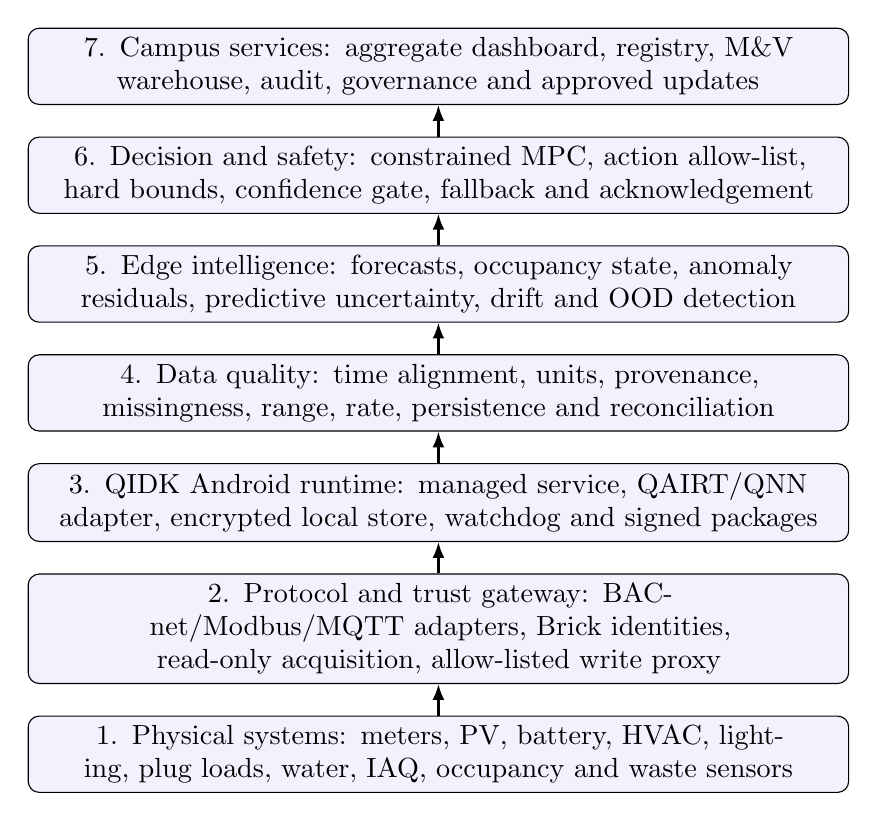
\begin{tikzpicture}[
		node distance=4mm,
		box/.style={draw,rounded corners,minimum height=8mm,text width=0.84\textwidth,align=center,fill=blue!5},
		arrow/.style={-{Latex[length=2mm]},thick}
		]
		\node[box] (physical) {1. Physical systems: meters, PV, battery, HVAC, lighting, plug loads, water, IAQ, occupancy and waste sensors};
		\node[box,above=of physical] (gateway) {2. Protocol and trust gateway: BACnet/Modbus/MQTT adapters, Brick identities, read-only acquisition, allow-listed write proxy};
		\node[box,above=of gateway] (android) {3. QIDK Android runtime: managed service, QAIRT/QNN adapter, encrypted local store, watchdog and signed packages};
		\node[box,above=of android] (quality) {4. Data quality: time alignment, units, provenance, missingness, range, rate, persistence and reconciliation};
		\node[box,above=of quality] (ai) {5. Edge intelligence: forecasts, occupancy state, anomaly residuals, predictive uncertainty, drift and OOD detection};
		\node[box,above=of ai] (decision) {6. Decision and safety: constrained MPC, action allow-list, hard bounds, confidence gate, fallback and acknowledgement};
		\node[box,above=of decision] (campus) {7. Campus services: aggregate dashboard, registry, M\&V warehouse, audit, governance and approved updates};
		\draw[arrow] (physical)--(gateway);
		\draw[arrow] (gateway)--(android);
		\draw[arrow] (android)--(quality);
		\draw[arrow] (quality)--(ai);
		\draw[arrow] (ai)--(decision);
		\draw[arrow] (decision)--(campus);
	\end{tikzpicture}
	\caption{\system{} architecture. Physical control remains in the existing BMS. Validated supervisory actions return from Layer 6 through the allow-listed Layer 2 gateway only in guarded closed-loop mode.}
	\label{fig:architecture}
\end{figure*}

\textbf{Layer 1, physical systems:} Revenue and building meters establish accounting boundaries. BMS points describe equipment operation but are not treated as revenue-grade energy evidence unless calibrated. Sensor placement, accuracy class, commissioning date, and maintenance status are retained.

\textbf{Layer 2, protocol and gateway:} A dedicated industrial gateway terminates BACnet/IP, BACnet/SC where available, Modbus, MQTT, and vendor interfaces. Shadow mode credentials are read-only. Closed-loop credentials can write only enumerated objects within priority and range rules. The QIDK device cannot directly scan or control the wider OT network. Brick classes and relationships map vendor point names to stable semantic identities~\cite{balaji2018brick}.

\textbf{Layer 3, Android runtime:} A managed foreground service coordinates acquisition, local storage, inference, scheduling, and health. Native C++ through the Android NDK/JNI hosts QNN. Android Keystore protects client credentials where the actual platform supports hardware-backed keys. A bounded local store permits at least 24 hours of disconnected operation and uses explicit retention classes.

\textbf{Layer 4, quality processing:} Every sample receives a source timestamp, receipt timestamp, engineering unit, quality code, and sequence number. Checks cover future timestamps, clock skew, impossible values, excessive rate of change, stuck sensors, duplicates, gaps, command/status disagreement, and meter hierarchy. Missingness indicators accompany imputation; no estimated interval is silently presented as measured.

\textbf{Layer 5, edge intelligence:} Separate model heads produce quantile forecasts of load, PV, occupancy, and thermal state. Deterministic and residual anomaly detectors operate before fusion. A drift service monitors input distributions, forecast residuals, missingness, and service outcomes. Models abstain outside the validated operating envelope.

\textbf{Layer 6, decisions and safety:} MPC proposes an action. A separate, non-learned kernel verifies data freshness, confidence, point authorization, physical range, rate, equipment state, minimum on/off times, and control mode. The gateway then performs a compare-and-write transaction and returns acknowledgement. A missing or inconsistent acknowledgement triggers fallback.

\textbf{Layer 7, campus services:} Cloud or campus servers may aggregate de-identified KPIs, train challengers, host a signed registry, and support M\&V. The real-time control path does not depend on these services.

\subsection{Operating-State Machine}

The deployment progresses monotonically only after review: \emph{replay} uses historical records; \emph{shadow} uses live data without visible action; \emph{advisory} exposes recommendations to operators; \emph{guarded closed loop} permits automatic bounded writes. Any stage may transition to fallback or safe stop. Model replacement returns the affected function to shadow mode, even if a previous model had closed-loop authorization.

\subsection{Trust Boundaries}

Four trust zones are defined: OT/BMS, the protocol gateway, QIDK analytics, and campus/cloud services. The gateway is the only component bridging QIDK and OT. External weather and carbon feeds are untrusted inputs: they are authenticated where possible, sanity-checked, timestamped, cached, and never permitted to override hard constraints. Model files are untrusted until signature, hash, schema, target-SoC, and runtime compatibility checks succeed.

\subsection{Edge Control Cycle}

\begin{algorithm}[t]
	\caption{Uncertainty-gated edge control cycle}
	\label{alg:control-cycle}
	\begin{algorithmic}[1]
		\Require telemetry $z_k$, safety policy $\Pi$, model $M$, previous action $u_{k-1}$
		\State validate signature, freshness, units, ranges and required channels
		\If{mandatory data invalid or platform not authorized}
		\State enter fallback and record reason
		\Else
		\State compute forecasts, intervals, anomaly and drift scores with $M$
		\If{uncertainty, drift or OOD exceeds validated threshold}
		\State enter fallback and record reason
		\Else
		\State solve constrained horizon problem for candidate $u_k^*$
		\State $u_k \gets \Pi(u_k^*,u_{k-1},z_k)$
		\If{$u_k$ rejected or solver deadline missed}
		\State enter fallback and record reason
		\ElsIf{mode is shadow}
		\State log $u_k$ without transmitting
		\ElsIf{mode is advisory}
		\State request operator approval
		\Else
		\State send $u_k$ through allow-listed gateway
		\State verify acknowledgement and observed response
		\EndIf
		\EndIf
		\EndIf
		\State append input, artifact hashes, decision and outcome to audit log
	\end{algorithmic}
\end{algorithm}

\section{Implementation Specification}

This section converts the architecture into testable component contracts. The implementation is intentionally small: the QIDK application, protocol gateway, model toolchain, and campus reporting service communicate through versioned records rather than shared internal state.

\subsection{Telemetry Contract}

Every observation is represented by the tuple
\begin{equation}
	z=\langle id,t_s,t_r,v,u,q,n,p\rangle,
\end{equation}
where $id$ is a stable semantic point identifier, $t_s$ source time, $t_r$ receipt time, $v$ value, $u$ engineering unit, $q$ quality code, $n$ sequence number, and $p$ provenance. Quality codes distinguish measured, estimated, missing, stale, out-of-range, and manually corrected records. Corrections append a new version and never overwrite the original.

The gateway converts source units to an agreed SI-oriented canonical form, while preserving the original value and unit for audit. A feature-schema manifest lists required and optional points, aggregation functions, look-back windows, permissible quality codes, normalization parameters, and feature order. A model cannot load if its feature-schema hash differs from the active manifest.

Telemetry is ingested at least once and deduplicated by source identity, timestamp, and sequence. Control does not rely on eventual deduplication: the current-state cache accepts only monotonic sequence numbers inside the clock-skew bound. Aggregation computes count, valid fraction, mean or integral, minimum, maximum, and last valid time so a plausible average cannot hide a severe short excursion.

\subsection{Forecast and Decision Contracts}

A forecast response contains target, issue time, valid-time vector, quantiles, physical bounds, model hash, calibration version, input-quality summary, out-of-distribution score, runtime backend, and elapsed time. Quantiles must be monotonic after post-processing. Negative load, PV beyond qualified capacity, impossible occupancy, and thermodynamically invalid states are rejected rather than clipped without a record.

The optimizer consumes only forecasts issued for the current cycle and returns a proposed trajectory, objective components before weighting, solver status, optimality or feasibility information, elapsed time, and fallback candidate. A single scalar objective is insufficient for audit because it can conceal a large service penalty behind an energy improvement.

A control proposal is
\begin{equation}
	a=\langle point,value,unit,start,expiry,priority,reason,h\rangle,
\end{equation}
where $h$ binds the proposal to its observation, forecast, model, optimizer, and safety-policy hashes. The gateway verifies these fields, current BMS mode, bounds and lease before writing. It returns accepted, rejected, superseded, timed-out, or indeterminate status together with the observed post-write value. Indeterminate is treated as failure, not success.

\subsection{Storage and Retention}

The QIDK store separates a current-state cache, short-term raw intervals, derived features, decisions, health events, and immutable audit summaries. Capacity is bounded by age and bytes. When disconnected, eviction removes the oldest non-audit raw records first; it cannot delete unresolved incidents or the records necessary to explain a control action. Once connectivity returns, aggregate upload uses resumable sequence ranges and verifies checksums.

Retention is purpose-specific. High-rate raw environmental and occupancy features receive the shortest operational period; aggregate resource intervals support M\&V; control and incident records remain for the approved audit period. Deletion is an explicit logged operation. Backups inherit the same expiry policy instead of retaining deleted personal data indefinitely.

\subsection{Control Transaction}

The write path uses a lease with a short expiry. At each cycle, the safety kernel evaluates the proposed action against point authorization, active building mode, manual override, physical and rate limits, minimum equipment times, data freshness, uncertainty, device health, and communication health. The gateway performs a conditional write only if the current BMS value and mode still match the state used by the optimizer. This prevents a delayed action from overwriting a recent operator command.

After writing, the platform verifies protocol acknowledgement and the resulting point value. It then observes the physical response over a defined confirmation interval. Failure to acknowledge, unexpected priority behavior, or movement in the wrong direction revokes the lease and invokes fallback. The BMS default sequence is sufficient to continue operation if QIDK disappears completely.

\subsection{Component Verification Matrix}

\begin{table*}[t]
	\centering
	\caption{Implementation verification matrix.}
	\label{tab:verification}
	\begin{tabularx}{\textwidth}{p{0.17\textwidth}p{0.25\textwidth}X p{0.18\textwidth}}
		\toprule
		Component         & Contract tests                                          & Fault and performance tests                                     & Release artifact                  \\
		\midrule
		Protocol adapters & Unit, timestamp, sequence, quality and identity mapping & Duplicate, reordering, gap, disconnect and malformed packet     & Point map and conformance log     \\
		Feature pipeline  & Deterministic replay and no-future-data check           & Missing channels, daylight-saving change and clock jump         & Schema and test vectors           \\
		Forecast runtime  & Reference numerical output and quantile order           & OOD, rare events, thermal soak and backend fallback             & Signed model card                 \\
		Optimizer         & Constraint and objective reconstruction                 & Infeasible state, timeout, forecast extremes and solver restart & Formulation and scenario suite    \\
		Safety kernel     & Boundary-value and authorization tests                  & Stale data, mode race, replay, corrupt policy and override      & Signed policy and coverage report \\
		Gateway writes    & Conditional write, lease and acknowledgement            & Lost acknowledgement, priority conflict and stale proposal      & Control matrix and HIL report     \\
		Local store       & Schema migration, checksum and deletion                 & Full disk, abrupt reboot and prolonged disconnection            & Retention and recovery report     \\
		M\&V ledger       & Meter and factor reconciliation                         & Missing intervals, factor revision and non-routine event        & Frozen ledger package             \\
		\bottomrule
	\end{tabularx}
\end{table*}

\subsection{Observability and Operations}

Health metrics include acquisition lag, valid-point fraction, queue depth, storage headroom, inference and solver latency, model abstention, drift state, backend, device temperature, process restarts, gateway round-trip time, write acceptance, overrides, and fallback reason. Alerts are rate-limited and grouped by root condition to avoid turning one network failure into hundreds of equipment alarms.

Operational dashboards distinguish measured physical outcomes from predictions and recommendations. They display active mode and authority, last successful cycle, current model and policy, data freshness, uncertainty, current constraints, recommended and issued actions, override state, and reason for fallback. A green status therefore means that a defined set of checks passed; it does not mean the building is net zero.

\section{Models and Optimization Methodology}

\subsection{Data Preparation and Leakage Prevention}

All model evaluation uses chronological splits. The final contiguous season or deployment period remains locked until model selection is complete. Scaling, missing-data models, feature selection, graph construction from statistical relationships, quantization calibration, and hyperparameter selection use training or validation data only. Weather inputs are the forecasts that would have been available at decision time, identified by issue timestamp; realized future weather is an oracle baseline, not a deployable feature.

Features include calendar and timetable, recent meter and equipment histories, forecast weather, aggregate occupancy state, tariff, carbon signal, and static semantic attributes. Missingness and quality are explicit features. Personally identifiable information is excluded. Daylight-saving transitions are represented in local time while storage and joins use UTC.

\subsection{Forecasting Candidates}

The following hierarchy prevents weak comparisons:
\begin{enumerate}[leftmargin=*]
	\item persistence, same-time previous day, and same-time previous week;
	\item regularized linear or generalized additive regression;
	\item gradient-boosted trees with lag and calendar features;
	\item compact TCN, N-BEATS, or TFT candidates;
	\item PatchTST and graph-temporal candidates; and
	\item frozen or fine-tuned Chronos, TimesFM, and Moirai challengers.
\end{enumerate}

For target $y$ and quantile $q$, models minimize pinball loss
\begin{equation}
	L_q(y,\hat y_q)=\max\{q(y-\hat y_q),(q-1)(y-\hat y_q)\}.
	\label{eq:pinball}
\end{equation}
Reported metrics include mean absolute error (MAE), root-mean-square error (RMSE), WAPE, normalized mean bias error (NMBE), coefficient of variation of RMSE (CVRMSE), empirical interval coverage, and interval width. Mean absolute percentage error is avoided where true load approaches zero.

\begin{align}
	MAE    & = \frac{1}{n}\sum_i|y_i-\hat y_i|,                      \\
	WAPE   & = 100\frac{\sum_i|y_i-\hat y_i|}{\sum_i|y_i|},          \\
	NMBE   & =100\frac{\sum_i(y_i-\hat y_i)}{(n-p)\bar y},           \\
	CVRMSE & =100\frac{\sqrt{\sum_i(y_i-\hat y_i)^2/(n-p)}}{\bar y}.
\end{align}

Forecast selection is based on downstream decision value as well as accuracy. A model that reduces WAPE but causes worse carbon, comfort, or actuator behavior in BOPTEST is rejected.

\subsection{Multimodal Fusion}

Meter, BMS, weather, and schedule features are aligned to a common interval and fused at feature level. Privacy-sensitive occupancy sensors produce local counts and confidence before fusion. Water and waste retain domain-specific temporal models because their event processes and sampling rates differ from HVAC. Campus graph nodes represent buildings, central plant, PV, battery, and shared meters; edges derive from documented physical or accounting relationships. A learned adjacency is allowed only as a labeled experiment.

\subsection{Anomaly and Fault Detection}

The first detector layer uses engineering tests: physical range, persistence, rate of change, redundant-sensor disagreement, energy balance, simultaneous heating/cooling, and command/status mismatch. The second layer uses standardized predictive residuals
\begin{equation}
	a_k=\frac{|y_k-\hat y_k|}{\hat\sigma_k+\epsilon}.
	\label{eq:anomaly-score}
\end{equation}
An alert requires persistence across a configurable window and valid upstream data. Precision, recall, $F_1$, false alarms per device-day, time to detection, and operator-confirmed diagnostic yield are reported. A high anomaly score is not labeled as a fault until evidence identifies a physical cause.

Water analytics detect improbable night flow, continuous flow, and main/submeter imbalance. Waste analytics forecast fill or collection demand and identify inconsistent weights or contamination records. These functions remain advisory in the pilot.

\subsection{Thermal and Resource Models}

A grey-box resistance-capacitance model is the primary thermal predictor because it is interpretable, compact, and suitable for MPC. Its discrete transition is
\begin{equation}
	\bm{x}_{k+1}=f_\theta(\bm{x}_k,\bm{u}_k,\bm{w}_k)+\bm{\epsilon}_k,
	\label{eq:dynamics}
\end{equation}
where $\bm{x}$ contains zone and envelope states, $\bm{u}$ approved setpoints or operating modes, and $\bm{w}$ weather, occupancy, solar and internal-gain forecasts. A learned dynamics model is evaluated as a challenger. Both are calibrated on training periods and checked on held-out extremes. A model validated for monthly energy is not assumed valid for 15-minute control.

\subsection{Carbon-Aware MPC}

At interval $k$, the controller solves a horizon $H$ problem:
\begin{align}
	\min_{\bm{u},\bm{\xi}} \sum_{j=0}^{H-1} [ & w_E\tilde E_{k+j}+w_C\widetilde{\gamma E}_{k+j}
	+w_P\tilde P_{k+j}^{peak}\nonumber                                                          \\
	                                          & +w_T\xi_{T,k+j}+w_Q\xi_{Q,k+j}
			+w_{\Delta u}\|\Delta\bm{u}_{k+j}\|_1].
	\label{eq:mpc-objective}
\end{align}
Tildes denote dimensionless normalized terms so weights are interpretable. All scales and weights are published. The optimization is subject to the dynamics in \cref{eq:dynamics}, approved actuator and rate constraints,
\begin{equation}
	\bm{u}^{min}\le\bm{u}_k\le\bm{u}^{max},\quad
	|\bm{u}_k-\bm{u}_{k-1}|\le\Delta\bm{u}^{max},
	\label{eq:actuator}
\end{equation}
and occupied comfort and IAQ constraints,
\begin{align}
	T_k^{min}-\xi_{T,k} & \le T_k\le T_k^{max}+\xi_{T,k},               \\
	c_k^{CO_2}          & \le c_k^{max}+\xi_{Q,k},\quad \bm{\xi}_k\ge0.
	\label{eq:service-constraints}
\end{align}
Slack is heavily penalized and independently alarmed. Exact limits come from applicable standards, equipment requirements, building use, and facilities approval; a universal temperature or \COtwo{} threshold is not assumed.

If a battery is present,
\begin{equation}
	s_{k+1}=s_k+\eta_cE_{ch,k}-\frac{E_{dis,k}}{\eta_d},
\end{equation}
with state-of-charge, reserve, power, efficiency, and cycling constraints. PV curtailment and export compensation are explicit rather than assumed.

\subsection{Uncertainty and Abstention}

Quantile forecasts, ensembles, or adaptive conformal residuals produce intervals. Scenario MPC evaluates sampled weather, occupancy, load, and PV trajectories. The controller abstains when empirical interval coverage falls below its validated bound, input shift exceeds threshold, required signals are stale, or the proposed trajectory reaches a prohibited state. Hard constraints remain active regardless of confidence.

\subsection{Drift and Updating}

Monitoring separates feature drift, missingness drift, residual drift, calibration drift, and physical outcome drift. A warning increases logging and forces advisory mode. Critical drift disables model control. Retraining is offline and cannot automatically overwrite the deployed champion. Every replacement receives chronological validation, numerical equivalence testing after conversion, artifact signing, and a new shadow period.

\subsection{Optional Federated Extension}

After two or more buildings have stable local models, personalized federated learning may share parameter updates without pooling raw occupancy or telemetry. The experiment compares local-only, pooled, FedAvg, and personalized heads. Secure aggregation and explicit client authentication are required. Differential privacy, if used, reports the complete $(\epsilon,\delta)$ budget and utility effect; the word ``private'' is not used merely because records remain local.

\section{Qualcomm QIDK Implementation}

\subsection{Hardware Qualification}

QIDK is a program and development target spanning premium Snapdragon Android platforms, not a single immutable SoC. Reproducibility therefore begins by recording the product identifier, board revision, SoC, CPU/GPU/Hexagon blocks, RAM, storage, Android build fingerprint and security patch, kernel, firmware, QAIRT/QNN version, thermal zones, power source, and device-management privileges~\cite{qualcomm_qidk}. The proposal will not transfer specifications from QCS6490 or RB5 to QIDK.

The qualification suite determines supported operators, tensor layouts, static or dynamic shapes, precision, backend fallback, initialization time, sustained thermal performance, memory, reboot recovery, and background-execution behavior. Advertised TOPS are not used as a proxy for application latency or efficiency.

\subsection{Software Components}

The Android application uses Kotlin or Java for lifecycle, health, configuration, and operator status; C++ through NDK/JNI for the QNN runtime; an encrypted bounded local database; and mutually authenticated HTTPS or MQTT to the gateway. WorkManager is reserved for deferrable work, not deterministic control timing. Continuous operation uses the managed-device facilities and foreground-service mechanisms supported by the qualified Android version.

The protocol gateway, not the application, hosts BACnet or Modbus authority. This reduces Android privileges and centralizes write-point enforcement. Application updates, models, safety policies, and feature schemas are separately signed and versioned. An atomic active/previous artifact arrangement supports rollback.

\subsection{Model Toolchain}

\begin{algorithm}[t]
	\caption{Training and QIDK packaging}
	\label{alg:packaging}
	\begin{algorithmic}[1]
		\State freeze chronological splits and feature schema
		\State train simple baselines and candidate models with fixed seeds
		\State calibrate uncertainty on validation data
		\State export candidate from PyTorch to supported ONNX representation
		\State verify framework and exported numerical outputs
		\State quantize using representative training-only calibration samples
		\State compile for available QNN targets and verify operator placement
		\State compare FP32/FP16/INT8 task metrics and calibration
		\State benchmark cold and steady latency, memory, temperature and energy
		\State create manifest with hashes, runtime, SoC and safety eligibility
		\State sign and deploy to shadow mode
	\end{algorithmic}
\end{algorithm}

The preferred path is PyTorch $\rightarrow$ ONNX $\rightarrow$ AIMET post-training quantization (PTQ) or quantization-aware training (QAT) $\rightarrow$ QAIRT/QNN compilation $\rightarrow$ Hexagon NPU. The GPU is evaluated for supported FP16 models and the CPU for preprocessing, control flow, optimization, unsupported operations, and deterministic fallback. QNN DLC may remain hardware-agnostic at the Qualcomm-runtime level; context binaries are treated as SoC-specific~\cite{qualcomm_aihub_compile}. Cloud AI Hub is optional and cannot receive sensitive proprietary models or calibration data without governance approval.

Representative calibration contains normal operations, peaks, low loads, season transitions, and known rare events. PTQ is attempted first. QAT is used only when PTQ violates an accuracy, calibration, or rare-event criterion~\cite{qualcomm_aihub_quant}. Mixed precision is not assumed to be supported by every Workbench or QNN release.

\subsection{Backend and Power Benchmark}

Each compatible backend and precision receives 100 warm-up executions and at least 1,000 measured batch-one executions. The report separates model initialization, cold inference, and thermal steady state. It includes median, p95, p99 and worst latency; peak resident memory; device temperature and frequency state; accelerator assignment; task error; and 24-hour stability.

Device power is measured with a calibrated external DC power analyzer between the supply and device input where hardware access permits. A synchronized marker brackets inference. Total and idle-subtracted energy are both reported:
\begin{equation}
	e_{inf}=\frac{\int_{t_0}^{t_1}[P_{active}(t)-P_{idle}(t)]dt}{N}.
\end{equation}
Screen, radio, camera, charge state, ambient temperature, and background tasks are fixed. Battery fuel-gauge readings may support diagnostics but do not replace external instrumentation. If the QIDK enclosure prevents direct supply measurement, the limitation and alternate measurement uncertainty are reported.

\begin{table}[t]
	\centering
	\caption{QIDK release gate for a model artifact.}
	\label{tab:qidk-gate}
	\begin{tabularx}{\columnwidth}{p{0.34\columnwidth}X}
		\toprule
		Gate          & Required evidence                                      \\
		\midrule
		Compatibility & SoC, QAIRT, firmware, schema and operator audit        \\
		Correctness   & Framework/export/device numerical comparison           \\
		Task quality  & Locked-test error, calibration and rare-event metrics  \\
		Timing        & Cold and sustained p50/p95/p99 latency                 \\
		Resources     & RAM, storage, initialization and thermal state         \\
		Energy        & Total and idle-subtracted energy per inference         \\
		Reliability   & 24-hour soak, reboot, WAN loss and corrupt-model tests \\
		Security      & Signature, hash, storage permissions and SBOM          \\
		Control       & Shadow evidence and safety approval                    \\
		\bottomrule
	\end{tabularx}
\end{table}

\subsection{Resilience}

The device caches at least 24 hours of approved schedules and the most recent valid external forecasts. Loss of WAN permits local inference and energy-only optimization only while cached inputs remain within freshness limits. Loss of the gateway, required sensor, model integrity, or time synchronization forces fallback. Reboot restores read-only operation until the service verifies artifacts, time, gateway identity, and current BMS state.

\section{Experimental Design}

\subsection{Stages and Experimental Units}

Evaluation proceeds from low to high physical risk. Historical replay checks leakage and metrics. BOPTEST and a calibrated twin test weather extremes, sensor faults, unavailable equipment, and forecast error. Hardware-in-the-loop (HIL) connects the real QIDK and gateway to simulated equipment. Live shadow and advisory stages then establish timing, operator interpretation, and drift behavior before guarded control.

The preferred field design uses comparable buildings or independently controlled zones in randomized week-long crossover blocks. Blocks are stratified by season, teaching versus vacation periods, and forecast weather. Washout is used when thermal or storage state carries treatment into the next block. If randomization is impossible, an interrupted time series with an untreated comparison building is used. Thousands of intervals from one building are not treated as thousands of independent experimental units.

\begin{table}[t]
	\centering
	\caption{Indicative evaluation stages.}
	\label{tab:stages}
	\begin{tabularx}{\columnwidth}{p{0.25\columnwidth}p{0.19\columnwidth}X}
		\toprule
		Stage              & Duration        & Promotion evidence                           \\
		\midrule
		Commissioning      & 4 weeks         & Meter, semantics and control matrix accepted \\
		Passive baseline   & 8--12 weeks     & Stable quality and baseline diagnostics      \\
		Replay and HIL     & 4--8 weeks      & Twin fault injection and deadline tests pass \\
		Shadow             & 4 weeks         & Reliable recommendations, no writes          \\
		Advisory           & 4 weeks         & Operator acceptance and reason codes         \\
		Closed-loop trial  & 12--24 weeks    & Registered sample and safety criteria        \\
		Seasonal extension & Up to 12 months & Annual coverage or stated projection         \\
		\bottomrule
	\end{tabularx}
\end{table}

\subsection{Comparison Arms}

Forecasting comparisons include persistence, daily and weekly seasonal forecasts, regularized regression, gradient boosting, the selected compact neural model, graph variants, and available foundation-model challengers. Control comparisons include existing BMS operation, facilities-tuned high-performance rules, energy-only MPC, carbon-aware MPC, and an oracle using realized future disturbances in simulation only. RL is a simulation comparator, never the sole physical baseline.

\subsection{Outcomes}

Three primary outcomes limit multiplicity: adjusted HVAC or whole-building energy, location-based operational emissions, and occupied comfort violation rate. Secondary outcomes are peak demand, cost, market-based emissions, IAQ violation time, forecast error and coverage, fault-detection yield, availability, overrides, data volume, latency, thermal throttling, and edge energy.

Occupied comfort violation rate is
\begin{equation}
	V_T=\frac{\sum_ko_k\mathbb{1}[T_k\notin[T_k^{min},T_k^{max}]]}{\sum_ko_k},
\end{equation}
where $o_k$ is an occupied indicator or weight. Peak reduction is
\begin{equation}
	R_{peak}=100\frac{P_{max}^{baseline}-P_{max}^{intervention}}{P_{max}^{baseline}}.
\end{equation}
The primary success condition is simultaneous improvement, not a weighted score that can hide harm:
\begin{align}
	\Delta E   & <0,          & \Delta C_{LB} & <0,          & S_E & >E_{platform},\nonumber \\
	\Delta V_T & \le\delta_T, & \Delta V_Q    & \le\delta_Q. &     &
\end{align}

\subsection{Ablations}

Offline and simulation ablations remove occupancy, weather forecast, carbon signal, uncertainty, graph edges, anomaly detection, drift gating, and the learned dynamics model. Hardware ablations compare CPU, GPU and NPU; FP32, FP16 and INT8; local and remote inference; forecast horizon; input resolution; and model size. Transfer ablations compare zero-shot, fine-tuned, building-specific, pooled, and personalized federated models. Safety gates are never removed in a physical closed-loop study.

\subsection{Statistical Analysis}

The randomization unit, seed, block schedule, exclusions, outcomes, model formulas, non-inferiority margins, and stopping conditions are registered before outcome unblinding. A fixed- or mixed-effects model estimates treatment effect:
\begin{equation}
	Y_{it}=\alpha_i+\lambda_t+\tau Z_{it}+\bm{\beta}^{\top}\bm{X}_{it}+\epsilon_{it},
	\label{eq:treatment}
\end{equation}
where $i$ is building or zone, $t$ time block, $Z$ treatment, and $\bm{X}$ predeclared weather, occupancy, and calendar covariates. Standard errors are clustered at the randomization unit. Effect sizes and 95\% confidence intervals accompany $p$-values. Comfort and IAQ use non-inferiority tests; secondary outcomes use Holm or false-discovery-rate correction.

Sensitivity checks include block bootstrap for autocorrelation, alternate weather specifications, complete-case and bounded missing-data treatments, placebo intervention dates, pre-trend tests, intention-to-treat and per-protocol effects, exclusion of approved non-routine events, and meter-uncertainty propagation.

A prospective power analysis uses baseline daily variance, intra-class correlation, autocorrelation, expected compliance, and minimum important effect. If the available units and duration cannot detect the planned 8\% energy effect, the study is labeled a feasibility study rather than an efficacy trial.

\section{Measurement, Verification, and Net-Zero Ledger}

\subsection{M\&V Plan}

The M\&V plan is approved before closed-loop operation. It identifies the measure, boundary, baseline and reporting periods, meter models and calibration, independent variables, model, routine and non-routine adjustments, missing-data procedure, expected savings relative to noise, uncertainty, reporting frequency, and persons authorized to approve changes. Whole-building impact uses an IPMVP Option C-style method. Separately metered HVAC or other measures use Option B. Calibrated simulation, corresponding to Option D, supports prospective scenarios but does not silently replace available measured evidence~\cite{ipmvp2022}.

The meter hierarchy is: utility revenue import/export; PV and battery; building main; HVAC, lighting, and plug-load submeters; QIDK and gateway power; then BMS points as secondary operational evidence. Interval totals are reconciled against utility bills. Data completeness is
\begin{equation}
	D_c=100\frac{N_{valid\ expected}}{N_{expected}},
\end{equation}
and submeter reconciliation error is
\begin{equation}
	R_e=100\frac{|\sum E_{submeters}-E_{main}|}{E_{main}}.
\end{equation}
Thresholds depend on meter criticality and are fixed during commissioning rather than borrowed as universal constants.

\subsection{Adjusted Baseline}

A baseline function estimates untreated energy using only causally prior variables:
\begin{equation}
	\hat E_k^{(0)}=f_\theta(T_k^{out},H_k,S_k,O_k,D_k,\tau_k),
\end{equation}
where $T^{out}$ is outdoor temperature, $H$ humidity, $S$ solar irradiance, $O$ occupancy proxy, $D$ day type, and $\tau$ time. The model is fitted before intervention analysis and checked for bias, CVRMSE, autocorrelation, heteroscedasticity, extreme-weather extrapolation, and seasonal residual patterns.

Avoided energy is
\begin{equation}
	S_E=\sum_{k\in\mathcal R}(\hat E_k^{(0)}-E_k^{(1)})\pm A_{nonroutine}.
\end{equation}
Its uncertainty is approximated and then checked by bootstrap:
\begin{equation}
	u(S_E)=\sqrt{u^2(\hat E^{(0)})+u^2(E^{(1)})+u^2(A_{nonroutine})}.
\end{equation}
Savings smaller than the practical detection limit are reported as inconclusive, not rounded into a positive claim.

Where a defensible comparison building exists, a difference-in-differences estimator is also reported:
\begin{align}
	\hat\tau_{DiD}={} & (\bar Y_{T,post}-\bar Y_{T,pre})\nonumber \\
	                  & -(\bar Y_{C,post}-\bar Y_{C,pre}).
\end{align}
Pre-intervention parallel trends are examined; DiD is not used when that assumption is implausible.

\subsection{Four Separate Ledgers}

\textbf{Site-energy ledger:} gross load, PV, storage charge/discharge and losses, imports, exports, curtailment, and platform consumption. The balance follows \cref{eq:energy-balance,eq:net-site}.

\textbf{Source-energy ledger:} site fuels multiplied by declared upstream conversion factors, if required by the institution. It is never labeled site energy.

\textbf{Location-based carbon ledger:} interval electricity multiplied by grid-average factors with source, region, vintage, issue time and units. Scope 1 fuels and refrigerants are separate. Export credit, if any, is disclosed rather than assumed.

\textbf{Market-based carbon ledger:} qualifying contractual electricity, residual mix, certificate serial numbers, technology, geography, vintage and retirement. It does not alter the physical energy ledger.

Avoided emissions, offsets, removals, and embodied hardware impacts are additional disclosures outside these ledgers. The platform cannot claim whole-campus net zero if material boundary sources are omitted.

\subsection{Water and Waste Verification}

Water main and submeters are reconciled, and leak alerts are evaluated against confirmed repairs and avoided-flow baselines. Weather and occupancy normalize irrigation and sanitary comparisons. Waste records reconcile scale tickets, stream classifications, rejected loads, and destinations. The platform reports total generation and prevention alongside diversion so a higher diversion percentage cannot conceal increased total waste.

\subsection{Factor Governance}

Each energy, carbon, water, and waste conversion factor retains publisher, dataset, release, geography, applicable period, unit, gas coverage and GWP basis, average or marginal interpretation, uncertainty, and fallback rationale. Historical results are recalculated only under a published policy. Marginal carbon forecasts may guide scheduling but remain separate from the location-based annual inventory~\cite{hawkes2010marginal,ghg_scope2}.

\section{Safety, Privacy, Security, and Governance}

\subsection{Safety Case}

The safety case argues from hazards to controls and evidence. Existing BMS and life-safety systems always override \system{}. The platform cannot write fire, smoke, emergency-power, access-control, elevator, or critical-process points. For permitted points, facilities staff approve absolute bounds, rate limits, minimum on/off periods, mode preconditions, priorities, and fallback values.

The independent safety kernel contains no learned policy. It validates action authorization and current physical context after optimization. A local emergency disable and gateway-side lease ensure that expired commands relinquish authority. HIL tests inject stale values, impossible states, clock jumps, duplicated packets, actuator failures, solver timeouts, model corruption, WAN loss, QIDK overheating, and reboot. Closed-loop eligibility is reviewed after every model, feature-schema, runtime, safety-policy, or writable-point change.

Incidents are classified by physical impact, service impact, security/privacy exposure, and recoverability. A Severity-1 event includes life-safety impact, equipment damage, or an uncontrolled prohibited action. Such an event stops the trial, preserves evidence, revokes write credentials, and requires independent review before any resumption.

\subsection{Privacy}

Privacy is based on minimization, purpose limitation, access restriction, and bounded retention rather than edge location alone. The data inventory records purpose, collection method, granularity, legal or ethical basis, access roles, storage location, retention, sharing, deletion, and consequences of error. Occupants receive understandable notice and a complaint channel.

Occupancy uses non-identifying environmental, mmWave, doorway-count, or schedule features where practical. If vision is indispensable and separately approved, frames remain in volatile local processing, only aggregate counts leave the sensor process, frames are immediately discarded, demographic performance is evaluated, and facial recognition is prohibited. Attendance, productivity, disciplinary, and individual trajectory inference are out of scope.

Fine-grained meter data can itself reveal occupancy and activity. External services therefore receive only the coarsest aggregate compatible with M\&V, and raw retention is shorter than KPI retention. Federated learning does not change these requirements.

\subsection{Cybersecurity}

The design follows OT principles from NIST SP 800-82 Rev. 3~\cite{nist80082}: network segmentation, least privilege, deny-by-default write access, authenticated devices, controlled remote access, secure configuration, monitoring, recovery, and attention to physical consequences. The QIDK, gateway, BMS, and campus services occupy separate network zones. Firewall rules identify exact peers, ports, and directions.

Transport uses mutual authentication where supported. Secrets use Android Keystore or an equivalent hardware-backed facility verified on the actual QIDK. Local data are encrypted; logs avoid raw tensors and credentials. Debug access is disabled in production. Applications, models, configurations, and safety policies are signed, hash-checked, versioned, and protected against unauthorized rollback. A software bill of materials (SBOM), vulnerability process, patch window, credential-rotation procedure, and decommissioning checklist are maintained.

The threat model covers malicious external feeds, replay, stale data, credential theft, rogue models, tampered updates, unauthorized BMS writes, denial of service, privacy inference, poisoned training data, federated clients, and physical access to the phone-class edge device. Secure boot or verified boot is used only if qualification confirms correct provisioning; its availability is not inferred from the Snapdragon brand.

\subsection{AI Governance}

Governance follows the NIST AI Risk Management Framework functions: Govern assigns authority and policy; Map documents context, affected people, and failure impact; Measure evaluates accuracy, calibration, drift, service and subgroup outcomes; Manage enforces release gates, monitoring, incident response, fallback and retirement~\cite{nistairmf}. ISO 50001 provides continual energy-performance management~\cite{iso50001}; ISO/IEC 42001 supplies an AI-management-system reference~\cite{iso42001}.

Each model has a model card describing purpose, prohibited use, training period, features, groups and seasons evaluated, metrics, uncertainty, hardware, runtime, energy, limitations, drift criteria, owner, and retirement date. Each dataset has a data sheet documenting collection, consent or authority, semantics, transformations, exclusions, missingness, privacy, and maintenance~\cite{mitchell2019modelcards,gebru2021datasheets}.

\begin{table*}[t]
	\centering
	\caption{Representative hazards, controls, and verification evidence.}
	\label{tab:hazards}
	\begin{tabularx}{\textwidth}{p{0.16\textwidth}p{0.26\textwidth}X p{0.18\textwidth}}
		\toprule
		Hazard                  & Preventive control                             & Detection and recovery                       & Evidence                           \\
		\midrule
		Unsafe setpoint         & Allow-list, hard range/rate, mode precondition & Gateway rejection, BMS override, fallback    & Boundary and fault-injection tests \\
		Stale or false sensor   & Freshness, plausibility, redundancy            & Quality alarm, abstention, approved schedule & Recorded fault replay              \\
		Model shift             & Locked operating envelope and no online update & Residual/coverage drift, shadow fallback     & Seasonal and OOD tests             \\
		Solver failure          & Deadline and feasible fallback trajectory      & Timeout before write                         & Worst-case timing test             \\
		WAN loss                & Cached approved inputs; no cloud dependency    & Freshness expiry, energy-only fallback       & 24-hour outage test                \\
		Device compromise       & Segmentation, least privilege, signing         & Revocation, isolation, forensic log          & Penetration and recovery exercise  \\
		Privacy leakage         & Local aggregation, retention limits            & Access audit and incident process            & Privacy impact assessment          \\
		Correlated fleet update & Canary release and compatibility manifest      & Health monitor and rollback                  & Fleet rollback drill               \\
		\bottomrule
	\end{tabularx}
\end{table*}

\section{Work Packages and Timeline}

The project is organized into ten dependent work packages over 22 months. Promotion criteria are evidence gates rather than target dates alone.

\begin{table*}[t]
	\centering
	\caption{Implementation work packages.}
	\label{tab:work-packages}
	\begin{tabularx}{\textwidth}{p{0.07\textwidth}p{0.1\textwidth}p{0.24\textwidth}X}
		\toprule
		WP & Months & Scope                                                                 & Acceptance criterion                                         \\
		\midrule
		1  & 1--2   & Scope, inventory boundaries, requirements, ethics and hazard analysis & Signed requirements, control exclusions and governance roles \\
		2  & 1--3   & QIDK/Android qualification and power method                           & Reproducible hardware/runtime report and soak test           \\
		3  & 2--5   & Metering, gateway, Brick graph and quality pipeline                   & At least 98\% valid critical intervals over 14 days          \\
		4  & 3--7   & Energy/carbon baselines and M\&V plan                                 & Frozen model passing predeclared residual diagnostics        \\
		5  & 4--8   & Forecasting, anomaly detection, uncertainty and quantization          & Candidate beats declared baselines and QIDK release gates    \\
		6  & 6--10  & Digital twin, MPC and independent safety kernel                       & BOPTEST and HIL fault suite pass                             \\
		7  & 9--12  & Live shadow and advisory deployment                                   & Stable availability; no uncontrolled writes                  \\
		8  & 12--18 & Registered randomized or crossover field trial                        & Sample, data quality and safety criteria met                 \\
		9  & 16--20 & Transfer, ablation, privacy and resilience studies                    & Locked cross-building and backend comparisons                \\
		10 & 19--22 & M\&V, audit, artifacts and dissemination                              & Independent reproducibility review and final release         \\
		\bottomrule
	\end{tabularx}
\end{table*}

Major milestones are: M1 scope approval; M2 privacy, security and safety review; M3 QIDK qualification; M5 telemetry commissioning; M7 frozen baselines; M9 HIL completion; M10 live shadow; M12 guarded-control readiness; M18 field-trial completion; M20 locked ledger; M21 reproducibility audit; and M22 final report and release.

Deliverables are: a boundary and governance specification; QIDK benchmark report; Brick point graph; versioned telemetry pipeline; baseline and predictive models; constrained optimizer and safety kernel; signed Android package; HIL suite; registered analysis plan; privacy-preserving research dataset; M\&V and net-zero ledger; model cards, data sheets, threat model and privacy assessment; reproducibility bundle; and final manuscript.

\subsection{Resource Plan}

Minimum roles are a principal investigator, building-controls engineer, Android/edge engineer, ML researcher, energy/M\&V analyst, data engineer, cybersecurity reviewer, privacy/ethics reviewer, and facilities operator. The pilot requires the QIDK target, managed Android support, industrial protocol gateway, meter access, calibrated device-level power analyzer, development server, test BMS or HIL interface, and approved access to weather and grid-factor data.

Procurement must include meter calibration and installation, gateway support, environmental sensors, secure mounting, power instrumentation, and software or standards access. The embodied impact and operational consumption of added equipment are recorded so the project does not externalize its own footprint.

\section{Risks, Limitations, and Expected Impact}

\begin{table*}[t]
	\centering
	\caption{Principal project risks and mitigations.}
	\label{tab:risks}
	\begin{tabularx}{\textwidth}{p{0.24\textwidth}p{0.11\textwidth}X}
		\toprule
		Risk                                               & Rating     & Mitigation                                                                   \\
		\midrule
		Required model operations unsupported on QIDK NPU  & M/M        & Operator audit, replacement, smaller model, graph partitioning, CPU fallback \\
		Android terminates long-running service            & M/H        & Managed device, supported foreground service, watchdog and restart test      \\
		Meter boundary cannot isolate impact               & H/H        & Commission early, add submetering, narrow claims to measured boundary        \\
		Short trial is mistaken for annual net zero        & H/H        & Label normalized projections; require complete ledger for achieved claim     \\
		Weather, timetable or operator confounding         & H/H        & Randomized blocks, comparison units, adjustments and override logs           \\
		Sensor drift or clock error                        & H/H        & Calibration, quality flags, cross-checks and time monitoring                 \\
		Occupancy processing creates privacy harm          & M/H        & Aggregate non-identifying sensors, local processing, impact review           \\
		Unsafe action                                      & L/Critical & Independent hard limits, BMS authority, HIL and staged release               \\
		Thermal throttling misses deadline                 & M/M        & Steady-state benchmark, cooling, compact model and CPU fallback              \\
		Carbon signal unavailable or inappropriate         & M/M        & Provenance and freshness checks; energy-only fallback                        \\
		Model drift                                        & H/M        & Coverage/residual monitoring, fallback and reviewed retraining               \\
		Savings below platform overhead or detection limit & L/M        & Measure overhead, simplify system and report inconclusive outcome            \\
		Cyber compromise                                   & L/Critical & Segmentation, least privilege, signed updates and incident exercise          \\
		Insufficient statistical power                     & M/H        & Prospective analysis, longer trial, more zones or feasibility classification \\
		\bottomrule
	\end{tabularx}
\end{table*}

The proposal has several inherent limitations. One campus cannot establish universal transferability. BOPTEST and a digital twin cannot prove field safety or savings. QIDK phones may not expose industrial power rails, long-term Android support, or the deterministic behavior of an embedded controller. Occupancy proxies may be biased or incomplete. Carbon-intensity data may be geographically coarse and revised after publication. A short pilot cannot assess full annual net-zero status or all Scope 3 emissions. These limitations are reported rather than concealed through broad claims.

If successful, the project contributes a reference pattern for resilient sustainability intelligence: data remain local where possible; cloud services become optional for immediate operation; predictive uncertainty affects authority; physical safety remains outside learned models; and environmental outcomes are measured against an auditable counterfactual. Operational deliverables can reduce energy, peak demand, emissions, water loss, false alarms, and external data movement. Scientific deliverables clarify when current forecasting SOTA adds control value on constrained edge hardware and whether its benefit exceeds compute energy and integration cost.

The project will not claim to be the first AI net-zero platform, guarantee emissions reduction, equate low average grid intensity with marginal impact, call federated learning private without additional controls, call a visualization a digital twin, or call simulation production validation. Its defensible contribution is the measured and governed integration of existing methods.

\section{Conclusion}

\system{} replaces a cloud-dependent monitoring-only model with distributed, bounded intelligence while retaining the BMS as physical authority. The proposed sequence begins with boundaries, meters, semantics, and deterministic checks; proceeds through forecasts, calibrated twins, and constrained MPC; and reaches physical control only after replay, HIL, shadow, advisory, and safety review. QIDK deployment is treated as a measured engineering problem involving model compatibility, quantization, thermal behavior, power, and recovery. The evaluation separates predictive accuracy from operational causality and separates site energy, location-based carbon, market-based carbon, and avoided emissions. This structure makes a negative or inconclusive result scientifically useful and prevents AI performance from being mistaken for verified net-zero progress.


\printbibliography

\appendices
\section{Notation and Metric Reference}

\begin{table*}[h]
	\centering
	\caption{Principal notation.}
	\label{tab:notation}
	\begin{tabularx}{\textwidth}{p{0.12\textwidth}p{0.52\textwidth}X}
		\toprule
		Symbol                 & Meaning                                                   & Unit                \\
		\midrule
		$k,\Delta t$           & Interval index and duration                               & --, h               \\
		$P,E$                  & Power and interval or accumulated energy                  & kW, kWh             \\
		$E_{grid,in/out}$      & Grid import/export energy                                 & kWh                 \\
		$E_{PV}$               & On-site photovoltaic generation                           & kWh                 \\
		$E_{bat,ch/dis}$       & Battery charge/discharge energy                           & kWh                 \\
		$A$                    & Gross floor area                                          & m$^2$               \\
		$\gamma$               & Electricity emissions factor                              & kg\,\COtwoe/kWh     \\
		$C_{S1},C_{S2}$        & Scope 1 and Scope 2 emissions                             & kg\,\COtwoe         \\
		$S_E,S_{net}$          & Gross avoided energy and savings net of platform energy   & kWh                 \\
		$\bm{x},\bm{u},\bm{w}$ & State, approved control and exogenous disturbance vectors & mixed               \\
		$H$                    & MPC prediction horizon                                    & intervals           \\
		$T,c^{CO_2}$           & Zone temperature and carbon-dioxide concentration         & $^\circ$C, ppm      \\
		$\xi_T,\xi_Q$          & Penalized comfort and IAQ slack                           & corresponding units \\
		$q$                    & Forecast quantile                                         & 0--1                \\
		$a_k$                  & Standardized anomaly score                                & dimensionless       \\
		$o_k$                  & Occupied indicator or weight                              & 0--1                \\
		$e_{inf}$              & Idle-subtracted energy per inference                      & J/inference         \\
		$u(\cdot)$             & Standard uncertainty                                      & corresponding units \\
		\bottomrule
	\end{tabularx}
\end{table*}

\subsection{Decision Threshold Register}

Before field operation, the team will publish a versioned register containing meter completeness, sensor freshness, clock skew, physical ranges, rate limits, forecast coverage, drift thresholds, solver deadline, setpoint bounds, equipment minimum times, comfort and IAQ constraints, non-inferiority margins, availability, latency, and incident severity. Each value identifies its source, rationale, approving role, effective date, and applicable operating mode. No threshold is silently changed during outcome analysis.

\subsection{Required Reporting Units}

Energy is reported in kWh and MWh with interval duration; power in kW; emissions in kg or t \COtwoe with GWP basis; water in L or m$^3$; waste in kg or t by stream; temperature in $^\circ$C; relative humidity in percent; \COtwo{} in ppm; particulate matter in \si{\micro\gram\per\cubic\meter}; latency in ms; energy per inference in J; memory in MiB; network volume in bytes; and area-normalized indicators per m$^2$. Conversions are versioned and applied once.

\section{Reproducibility Protocol}

The release supports five levels: regenerate all figures from released aggregates; retrain models on an approved anonymized or synthetic dataset; reproduce QIDK benchmarks on equivalent hardware; replay the controller against recorded telemetry; and conduct site-specific deployment only after a new safety review.

\subsection{Hardware Manifest}

The manifest records QIDK product and board identifiers, SoC, RAM and storage, power configuration, Android build fingerprint, security patch, kernel, firmware, gateway and meter models, sensor placement and calibration, network topology, and power-analyzer method. Diagrams omit credentials and exploitable addressing.

\subsection{Software Manifest}

The manifest records source revision, Android Gradle Plugin, SDK/NDK, Java/Kotlin and C++ toolchains, QAIRT/QNN and firmware versions, training lockfile or container digest, compiler flags, model and configuration hashes, feature schema, solver version, signed-package identifiers, SBOM, and licenses.

\subsection{Data Manifest}

The data dictionary identifies every point, Brick mapping, unit, source rate, aggregation, timezone and daylight-saving rule, missingness code, calibration period, intervention label, exclusion, privacy transformation, retention class, dataset version, and checksum. Raw identity-bearing data are not released. A synthetic or statistically protected substitute accompanies restricted operational data.

\subsection{Experiment Manifest}

The registered record includes randomization unit, blocks, seed and schedule; train/validation/test dates; hyperparameter search; final seeds; quantization calibration IDs; stopping and exclusion rules; primary and secondary outcomes; statistical formulas; software versions; intervention approvals; non-routine events; and exact commands required to regenerate tables and figures.

\subsection{Final Audit Checklist}

An independent reviewer must be able to determine from the artifacts: the exact claimed boundary; supporting meters; model inputs and outputs; permitted and prohibited actions; failure behavior; counterfactual baseline; experimental unit; comfort and IAQ protection; edge-energy treatment; carbon-factor provenance; artifact lineage; and conclusions that remain invalid without a complete annual trial. Failure to answer any item blocks final release.


\end{document}
